% NOTE: source arXiv 2505.22954 presents this figure and
% figures/02_dgm_comparisons_polyglot.tex as two subfigures of one combined
% float (single shared caption, labels fig:dgm-comparisons-swe /
% fig:dgm-comparisons-polyglot, neither individually \Cref'd — only the
% outer \label{fig:dgm-comparisons} is referenced in the paper body). Split
% into two single-asset floats to satisfy paper/figures/README.md's
% one-wrapper-per-one-asset convention; this wrapper keeps the
% paper-referenced label. See paper/supplementary/source-attribution.md.
\begin{figure}[ht]
\centering
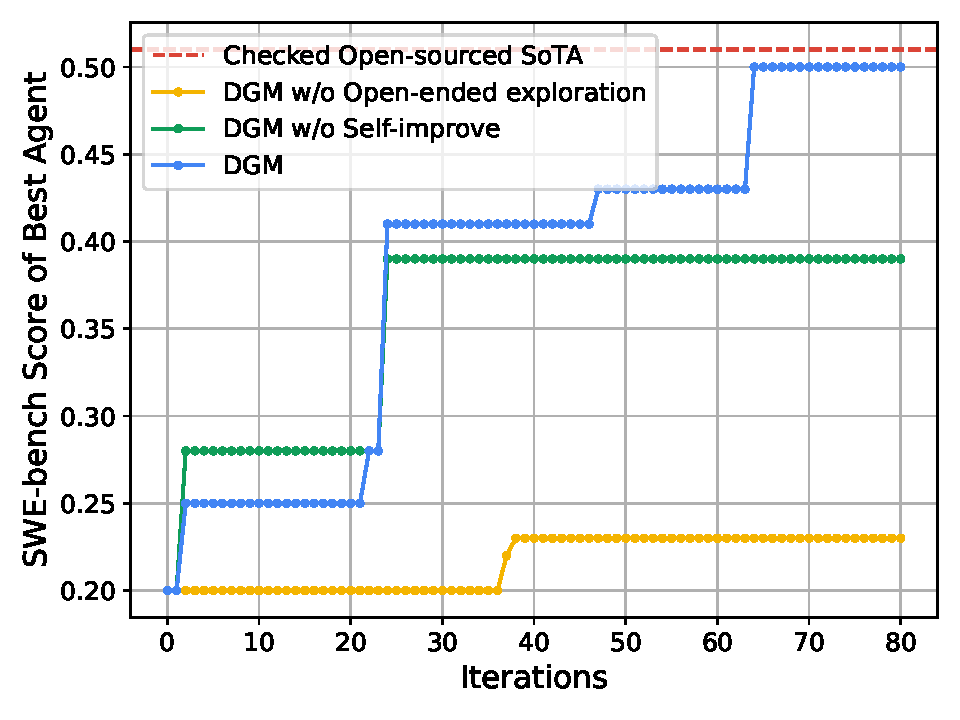
\includegraphics[width=0.7\textwidth]{figures/srcs/01_dgm_comparisons_swe.pdf}
\caption{\textbf{Self-improvement and open-ended exploration enable the DGM to continue making progress and improve its performance.} The DGM automatically discovers increasingly better coding agents and performs better on both (Left) SWE-bench and (Right) Polyglot. It outperforms baselines that lack either self-improvement or open-ended exploration, showing that both components are essential for continual self-improvement. These scores are obtained from evaluating on the benchmark subsets detailed in \Cref{sec:benchmarks}. (SWE-bench panel; see \Cref{fig:dgm-comparisons-polyglot} for the paired Polyglot panel.)}
\label{fig:dgm-comparisons}
\end{figure}
